% !TeX spellcheck = pt_BR


\chapter{A demonstração geral do Teorema da Energia Cinética} \label{apendice-teoremaenergiacinetica}



No texto principal, demonstramos o Teorema Trabalho-Energia --- ou Teorema da Energia Cinética (Equação \ref{eq_energia_teoremaenergiacinetica}) --- para o caso em
que a força resultante é constante, que acarretava um MUV. O resultado foi:

$$ W = F \cdot d = ma \cdot d = m \cdot \frac{v^2 - v_0^2}{2} = \Delta E_c. $$

A demonstração usou a Equação de Torricelli $v^2 = v_0^2 + 2ad$, que só vale para aceleração constante. Quando a força varia ao longo do deslocamento, essa equação não
pode ser usada diretamente --- e surge a pergunta natural: o teorema ainda
vale?

A resposta é sim. E a demonstração usa exatamente o mesmo argumento de
fatiamento do Apêndice~\ref{apendice_areagraficovxt}, com uma surpresa
algébrica no meio.


A estratégia é aplicar o resultado já conhecido a cada fatia. Dividimos o deslocamento total em $n$ fatias muito pequenas, de comprimento
$\Delta x_i$ cada. Em cada fatia, a força mal varia --- é como se fosse
constante. Sendo constante naquela fatia, a aceleração também o é:
$a_i = F_i/m$. E sendo a aceleração constante em cada fatia, podemos usar
a equação do MUV localmente:

$$ v_{i+1}^2 = v_i^2 + 2\,a_i\,\Delta x_i
   \;\;\Longrightarrow\;\;
   a_i\,\Delta x_i = \frac{v_{i+1}^2 - v_i^2}{2}, $$

   \noindent em que $v_i$ é a velocidade inicial, no início do deslocamento, e $v_{i+1}$ é a velocidade final após percorrer a fatia de comprimento $\Delta x_i.$

O trabalho realizado pela força nessa fatia é

$$ \Delta W_i = F_i \cdot \Delta x_i = m\,a_i\,\Delta x_i
   = \frac{m}{2}\!\left(v_{i+1}^2 - v_i^2\right). $$


Note que $\Delta W_i = F_i \Delta x_i$ é a área de um retângulo de altura $F_i$ e largura $\Delta x_i$, como mostra a primeira imagem da Figura \ref{fig_apendice_area_teoremaEc}. Assim, ao fatiar os deslocamentos, o trabalho em cada trecho é a área do retângulo abaixo da curva no gráfico de $F$ por $x$, de modo que o trabalho total é a área total abaixo do gráfico, como mostram as duas outras imagens da figura.

A equação anterior mostra que cada fatia contribui com um trabalho igual a uma diferença de velocidades ao quadrado, multiplicada
por $m/2$. Até aqui, nenhuma surpresa. A surpresa vem quando somamos tudo.



\vspace{0.3cm}
{
\centering
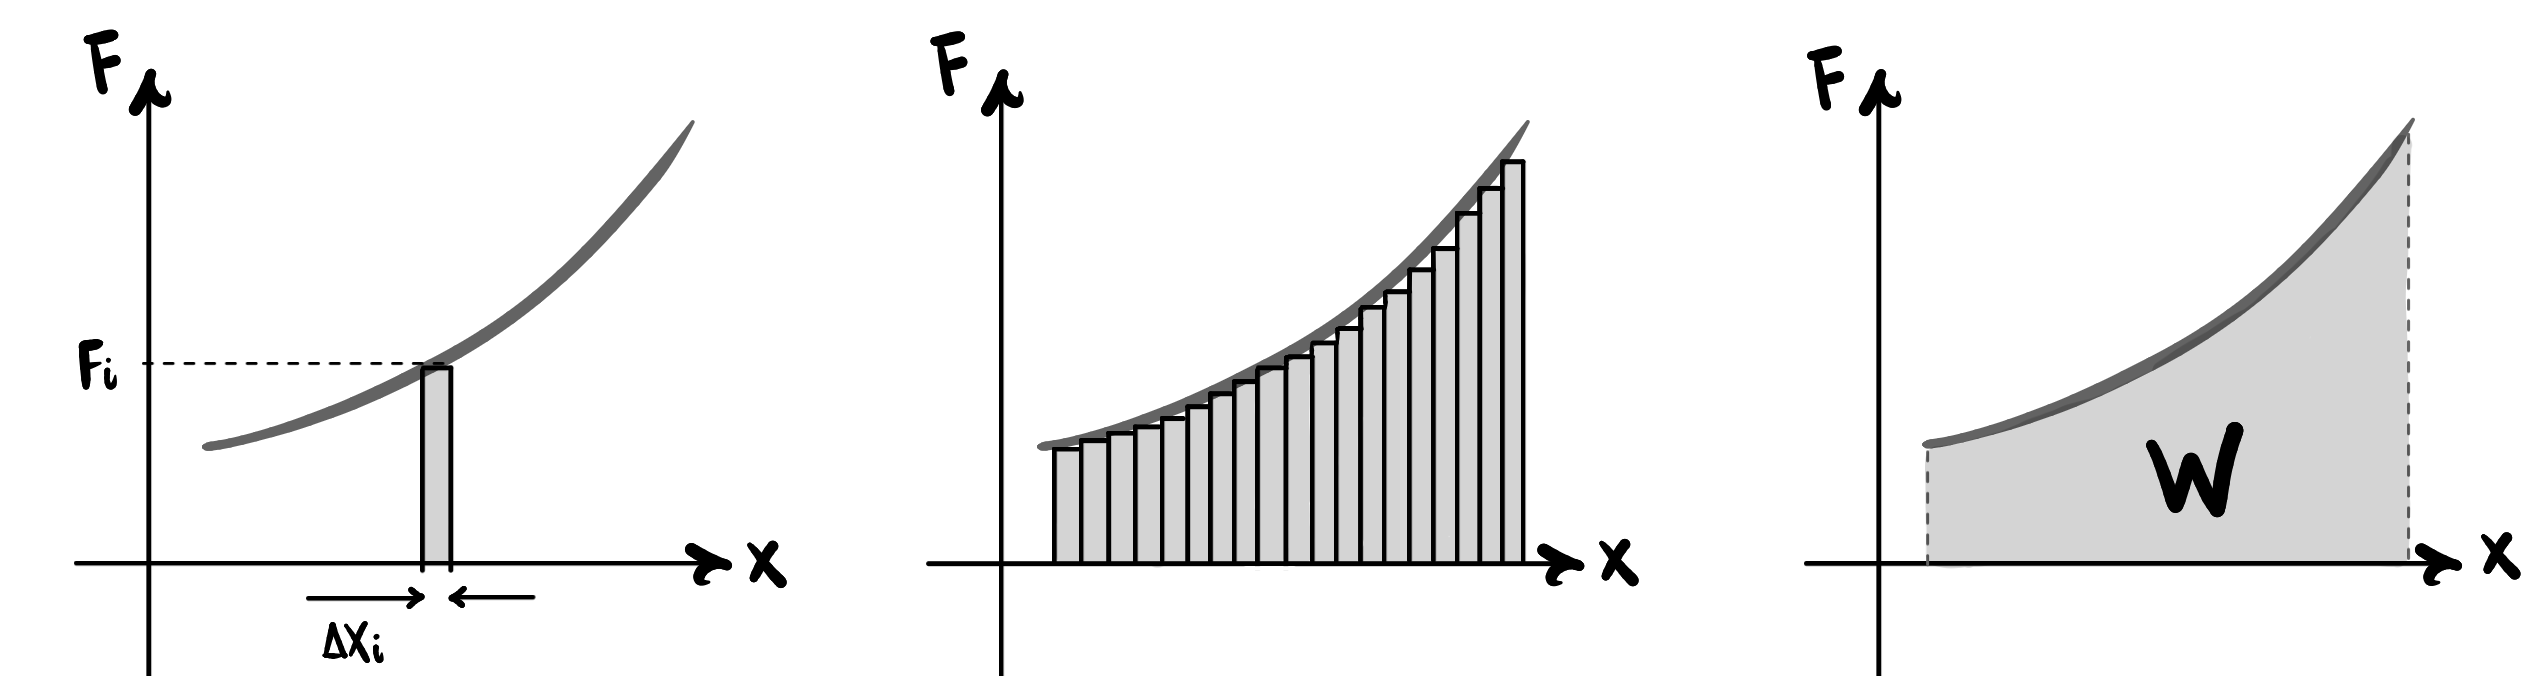
\includegraphics[width=0.95\linewidth]{imagensapendices/teoremaenergiacinetica.png}
\captionof{figure}{A força $F$ varia ao longo do deslocamento $x$. Em cada fatia a velocidade muda de $v_i$ para $v_{i+1}$ e o trabalho nesse trecho vale $\Delta W_i = F_i \Delta x_i = \frac{m}{2} (v_{i+1}^2 - v_{i}^2)$. }
\label{fig_apendice_area_teoremaEc}
} 
\vspace{0.3cm}





O trabalho total da força ao longo do deslocamento é a soma de todas as contribuições (soma das áreas dos retângulos):

$$ W = \sum_{i=1}^{n} \Delta W_i
     = \frac{m}{2}\sum_{i=1}^{n}\!\left(v_{i+1}^2 - v_i^2\right). $$

Escrevendo os termos um a um:

$$ W = \frac{m}{2}\Big[
    \left(v_1^2 - v_0^2\right)
  + \left(v_2^2 - v_1^2\right)
  + \left(v_3^2 - v_2^2\right)
  + \cdots
  + \left(v_n^2 - v_{n-1}^2\right)
  \Big]. $$

Observe que $v_1^2$ aparece com sinal positivo no primeiro parênteses e com sinal
negativo no segundo; $v_2^2$ aparece positivo no segundo e negativo no
terceiro; e assim por diante. Todos os termos intermediários se cancelam.
Sobram apenas o primeiro e o último:

$$  W = \frac{m}{2}\!\left(v_n^2 - v_0^2\right)
      = \frac{1}{2}mv_n^2 - \frac{1}{2}mv_0^2. $$


Assim, o Teorema da Energia Cinética vale para qualquer força, constante ou variável:
$$ W = \Delta E_c = E_{c_\text{FINAL}} - E_{c_\text{INICIAL}}. $$



Cabe destacar aqui alguns pontos. A prova tem dois momentos distintos. O primeiro é o argumento das fatias ---
o mesmo do Apêndice~\ref{apendice_areagraficovxt}: em cada intervalo pequeno,
a força é localmente constante, então o resultado já demonstrado para o MUV
se aplica. Até aqui, tudo é aproximado.

O segundo movimento é puramente algébrico, e é exato: a soma telescópica.
Cada velocidade intermediária $v_i$ aparece exatamente duas vezes na soma
--- uma com sinal positivo e uma com sinal negativo --- e portanto some.
O resultado final depende apenas de $v_0$ e $v_n$; todo o caminho percorrido
entre eles, com toda a complexidade da variação de $F$, desaparece.

Isso é uma primeira e poderosa antecipação de por que os métodos energéticos
são tão úteis na mecânica: eles ignoram os detalhes intermediários e enxergam
apenas o estado inicial e o estado final, como já destacamos anteriormente. Uma força que varia de forma
arbitrariamente complicada ao longo de uma trajetória tem um único número
associado a ela --- o trabalho --- e esse número determina completamente a
variação de energia cinética do corpo. O caminho some; o resultado fica.